\documentclass[a4paper]{article}

\usepackage{graphicx}
\usepackage{amsmath,amssymb}
\usepackage{minted}
\usepackage{multirow}
\usepackage{float}
\usepackage{algorithm}
\usepackage{algpseudocode}
\usepackage{todonotes}
\usepackage{forest}
\usepackage{xstring}
\usepackage{xcolor}
\usepackage[most]{tcolorbox}
\usepackage{xparse}
\usepackage{natbib}
\usepackage{adjustbox}

\usetikzlibrary{graphs,graphdrawing}
\usegdlibrary{layered}

% for external graphviz
\input{/home/donkarlo/Dropbox/repo/nd_language_ai_project/src/nd_language_ai/formal/computer/programming/tex/latex/code_clips/external_graphviz.tex}

% for tags
\input{/home/donkarlo/Dropbox/repo/nd_language_ai_project/src/nd_language_ai/formal/computer/programming/tex/latex/part/control_sequence/kind/semtag/semtag.tex}

% for links
\input{/home/donkarlo/Dropbox/repo/nd_language_ai_project/src/nd_language_ai/formal/computer/programming/tex/latex/code_clips/seehere.tex}

% for nested lists and sections
\input{/home/donkarlo/Dropbox/repo/nd_language_ai_project/src/nd_language_ai/formal/computer/programming/tex/latex/code_clips/deep_structure.tex}

\title{}
\date{}
\author{Mohammad Rahmani}

\begin{document}
   \maketitle
   \seeherefooter{}
   \begin{figure}[H]
      \centering
      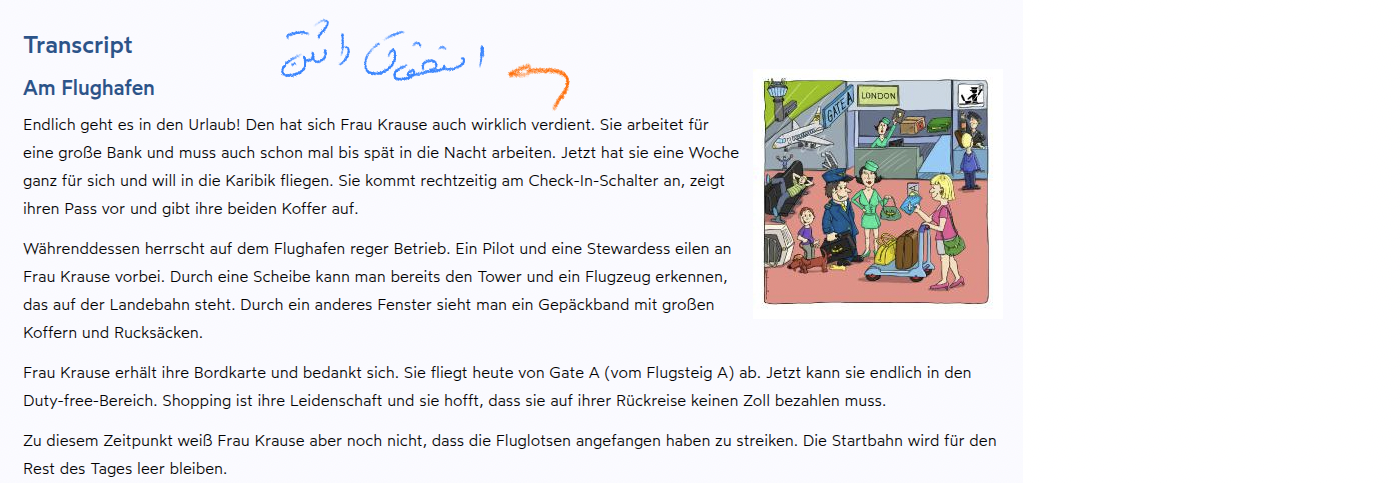
\includegraphics[width=0.9\textwidth]{img_1.png}
   \end{figure}
   \section{ترجمه انگلیسی}
      بالاخره زمان رفتن به تعطیلات فرا رسیده است! خانم کراوزه واقعاً هم شایستهٔ این تعطیلات است. او در یک بانک بزرگ کار می‌کند و گاهی مجبور است تا دیروقتِ شب کار کند. حالا یک هفته را کاملاً برای خودش در اختیار دارد و می‌خواهد به منطقهٔ کارائیب پرواز کند. او به‌موقع به پیشخوان پذیرش پرواز (Check-in) می‌رسد، گذرنامه‌اش را نشان می‌دهد و دو چمدانش را تحویل می‌دهد.

      در همین حین، فرودگاه بسیار شلوغ و پرجنب‌وجوش است. یک خلبان و یک مهماندار هواپیما باعجله از کنار خانم کراوزه عبور می‌کنند. از پشت یک شیشه می‌توان برج مراقبت و هواپیمایی را دید که روی باند فرود ایستاده است. از پنجره‌ای دیگر، نوار نقالهٔ حمل بار را می‌توان دید که چمدان‌ها و کوله‌پشتی‌های بزرگی روی آن قرار دارند.

      خانم کراوزه کارت پروازش را دریافت می‌کند و تشکر می‌کند. پرواز او امروز از گیت A (خروجی A) انجام می‌شود. حالا بالاخره می‌تواند وارد بخش فروشگاه‌های معاف از عوارض گمرکی (Duty-free) شود. خرید کردن علاقهٔ شدید اوست و امیدوار است که هنگام بازگشت از سفر مجبور نباشد هیچ عوارض گمرکی پرداخت کند.

      اما در این لحظه، خانم کراوزه هنوز نمی‌داند که خلبانان شرکت‌های هواپیمایی اعتصاب خود را آغاز کرده‌اند. باند پرواز تا پایان روز خالی خواهد ماند.
      \begin{figure}[H]
         \centering
         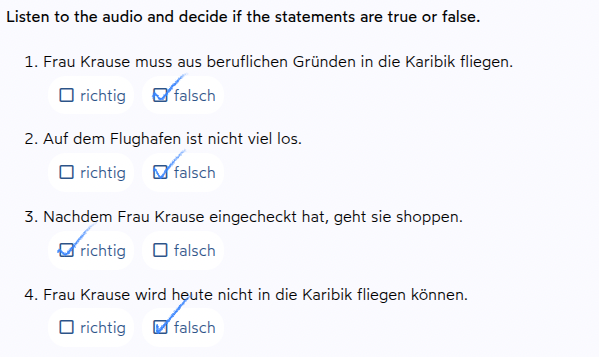
\includegraphics[width=0.9\textwidth]{img_0.png}
      \end{figure}

      \bibliographystyle{plainnat}
      \bibliography{/home/donkarlo/Dropbox/repo/nd_shared_research/bibliography/bibliography.bib}
\end{document}
